It has been proven that the climate change, among other environmental challenges, is (mostly) due to the concentration of anthropogenic \gls{GHG} in the environment \cite{IPCC_CO2_budget}. Therefore, the \gls{GHG} emissions from human activities must be mitigated to prevent further environmental damages. Among these emissions, globally, about 75\% are directly related to the whole-energy system \cite{ourworldindata_CO2_world}. The \gls{GHG} emissions usually expressed in kt$_{\ce{CO2},\text{eq}}$, could be developed as an adapted, \ie less economy-oriented, version of the original Kaya identity \cite{kaya1997environment}:

\begin{equation}
\label{eq:equality_GHG}
\mathrm{GHG} =  \frac{\mathrm{GHG}}{\text{Primary energy}} \times \frac{\text{Primary energy}}{\mathrm{EUD}}\times \frac{\mathrm{EUD}}{\text{Population}} \times \text{Population}\\
 \end{equation}

\noindent
where the first term represents the \gls{GWP} of the primary energy mix, the second is the inverse of the efficiency and the third could stand as the energy intensity per capita. Such an identity, mathematically-correct though, is criticized for the arbitrary choice of variables, the non-independence of them usually leading to the rebound effect and its global/encompassing approach that does not translate properly the heterogeneity of the situation \cite{IPCC2000}. However, Eq. \ref{eq:equality_GHG} has the merit to highlight three levers of action that should be activated to reduce the \gls{GHG} emissions and, consequently, favour the transition, leaving aside the question of the total population and its growth \cite{dodson2020population,scovronick2017impact}. These three levers of actions are: renewables, efficiency and sufficiency aiming at reducing the first, the second and the third terms on the right-hand side of Eq. \ref{eq:equality_GHG}, respectively. The latter, explicitly mentioned by the IPCC for the first time in 2022 \cite{IPCC2022}, is defined by \citet{lage2023citizens} as ``a strategy for reducing, in absolute terms, the consumption and production of end-use products and services through changes in social practices in order to comply with environmental sustainability while ensuring an adequate social foundation for all people''. Altough this finds a growing interest in the scientific community \cite{o2018good}, it requires, maybe more than the two other levers, interdisciplinarity \cite{schmidt2015interdisciplinary}, \ie the combination of multiple academic disciplines like sociology, psychology or politics, that are out of the scope of my expertise, and, consequently, this thesis. However, the work developed in the present manuscript aims at providing support to such interdisciplinary projects to assess sufficiency policies. More within the grasp of the engineering world, this thesis rather focuses on the first two terms of Eq. \ref{eq:equality_GHG}, \ie renewables and efficiency. This aligns with the current European policies binding the Member States of the European Union. For instance, the Renewable Energy Directive (RED) III, published in October 2023 \cite{REDIII}, highlights that ``the Union’s climate neutrality objective (by 2050) requires a just energy transition which leaves no territory or citizen behind\footnote{This directly relates to sufficiency as it encompasses social justice in parallel with a minimization of the energy use.}, an \textbf{increase in energy efficiency} and significantly \textbf{higher shares of energy from renewable sources} in an integrated energy system'' (\ie 42.5\% of the Union's gross final consumption of energy by 2030). 

Consequently, to ensure the energy supply of an assumably more and more demanding society in a context of environmental crisis, major transformations are needed (see Figure \ref{fig:intro:IEA_WEO_2019}). Besides behavioral changes, an overall reshape of the energy system is necessary in terms of both primary energy sources, \ie more renewables, and technologies used to convert these resources into the \gls{EUD} (\ie the energy service required by the the final consumer), \ie more efficiency \cite{iea2020world,luderer2018residual}. The former corresponds to a whole ``fuel switch'' (see Figure \ref{fig:intro:IEA_WEO_2019}) where energy carriers called, in the literature, ``\emph{biofuels}'', ``\emph{electrofuels}'', ``\emph{synthetic fuels}'', ``\emph{renewable fuels}'' or even ``\emph{sustainable fuels}'', will more and more play a crucial role. To avoid the confusion between these fuels and thereby reduce misunderstanding in political or academic discussions, we have suggested a comprehensive and harmonised taxonomy (see Appendix \ref{app:Taxonomy}). In the rest of this thesis, the electro - and bio - fuels are considered as renewable and with no \gls{GWP}.  

\begin{figure}[ht!]
\centering
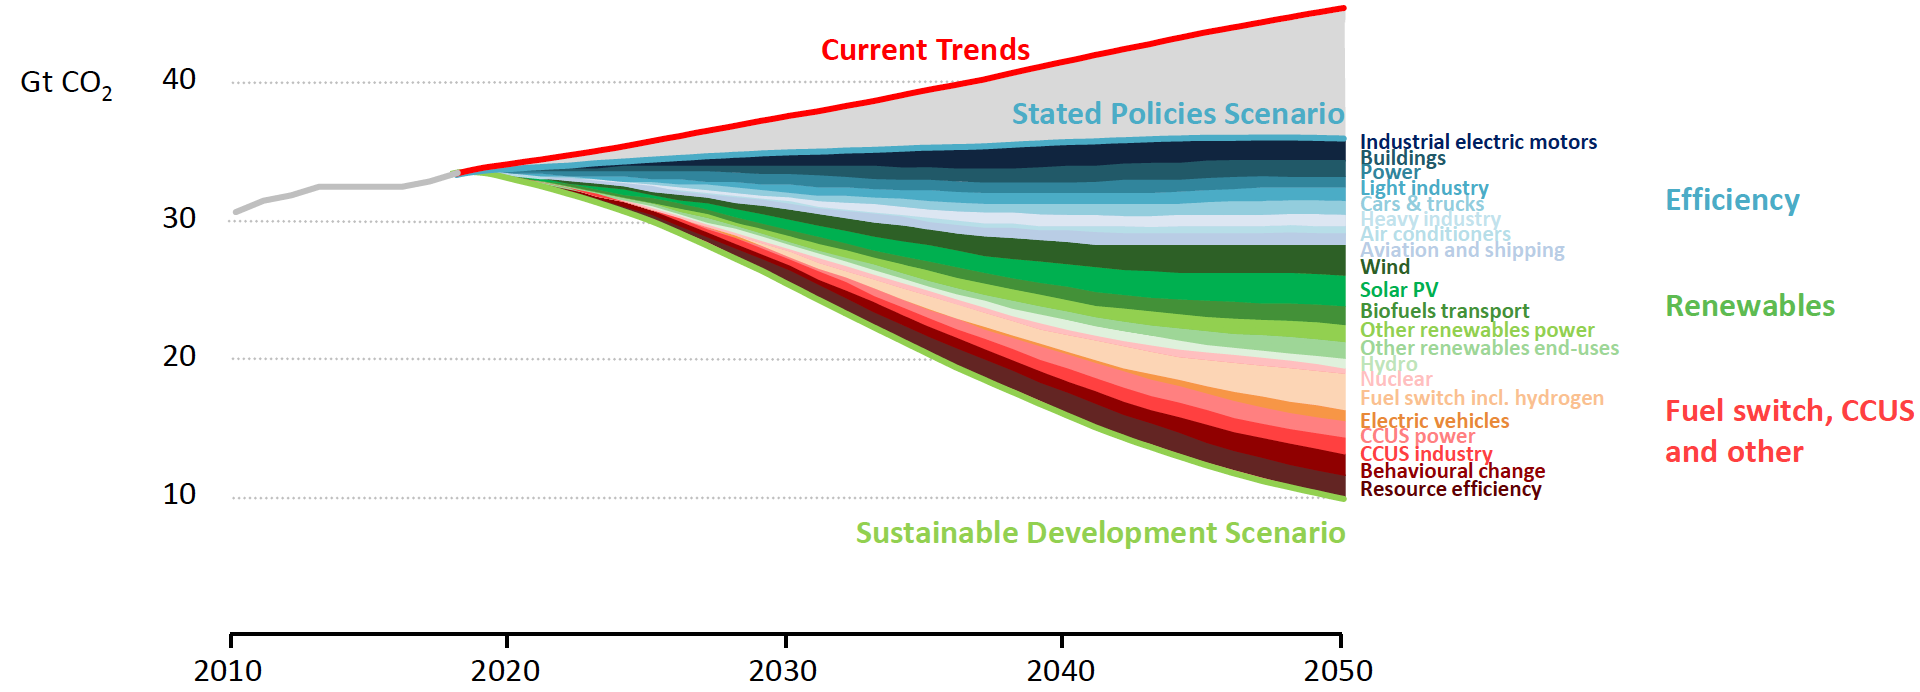
\includegraphics[width=\textwidth]{IEA_WEO_2019.png}
\caption{Energy-related CO2 emissions and reductions by sources in the Sustainable Development Scenario \cite{iea2020world}.}
\label{fig:intro:IEA_WEO_2019}
\end{figure}

In the general perspective to decrease the \gls{GWP} of the primary energy mix, \gls{VRES} like wind and solar, have already emerged as the keystone to defossilise the energy system. However, their intermittency and space disparity could hold back their vaster integration in the future. To address this issue, due to some limitations (\eg range, power, costs) of electricity-focused solutions like \gls{DC} lines, the transport and long-term storage of the renewable electricity produced in excess should be optimised.

This challenge can be tackled by \textit{electrofuels} \cite{rozzi2020}. These fuels represent energy carriers where electricity has the major share in the energy balance of the fuel. In practice, this electricity is mainly converted into hydrogen (\ie electrolysis) and then potentially upgraded into more complex fuels (\eg methane, methanol or ammonia). Even if the share of electricity increases in the energy system through the electrification of the end-use demand, gaseous and liquid fuels will keep on being big players during (and after) the energy transition \cite{Ahlgren2012}. They offer three main advantages: infrastructure compatibility, storage and capacity to link sectors (\ie from electricity to mobility, heat, or industry). Development on electrofuels aims at getting them more and more compatible with existing and mature technologies \cite{Ahlgren2012}. An example is carbon-free ammonia-hydrogen blends burned in spark ignition engines \cite{lhuillier2020experimental} or \gls{CHP} applications \cite{pochet202022}. With a growing share of \gls{VRES}, sector coupling is essential to absorb the surplus of electricity from these intermittent production means \cite{robinius2017linking} and integrate them more cost-effectively \cite{brown2018response, limpensECOS2021}. Besides direct electrification of other sectors (\eg electrical heat pumps, battery electric vehicles), \citet{brown2018synergies} showed that converting power to hydrogen and methane was advantageous at high shares of renewables, in their optimisation of the European whole-energy system. Electrofuels have the ability to couple energy and non-energy sectors \cite{Stancin2020}. For instance, electricity produced in excess from \gls{VRES} can be converted in ammonia through the Haber-Bosch process and subsequently transformed into fertiliser - coupling the power and industry sectors \cite{verleysen2020can}. Gas networks present much more storage potential than electrical network (\eg 50 times more in Germany and 300 times more in France) \cite{Rosa2017}. Where batteries exhibit limited storage capacity (up to 10\,MWh) as well as self-discharge losses, electrofuels are an economical solution for high capacity (from 100 GWh) and long-term (\ie from months to years) storage of energy \cite{child2018role, dias2020energy} (see Figure \ref{fig:intro:Storage_electrofuels}.) Besides storing energy, in their analysis of the German transport sector in 2050, \citet{millinger2021electrofuels} highlighted that producing electrofuels can represent a better usage of the ambient \ce{CO2} than \gls{CCS} to supply hydrocarbon fuels while limiting the curtailment of \gls{VRES}. Moreover, some applications (\eg marine, aviation and heavy-duty transport) will be hard to electrify and keep on requiring high-density energy carriers \cite{horvath2018techno, brynolf2018}. These carriers, currently produced mostly from fossil resources, will still consist of hydrocarbons in a renewable world. This is why this paper rather uses "defossilisation" rather than "decarbonisation" as carbon will still play a key role in a carbon-neutral energy transition \cite{mertens2020carbon}.

\begin{figure}[htbp!]
\centering
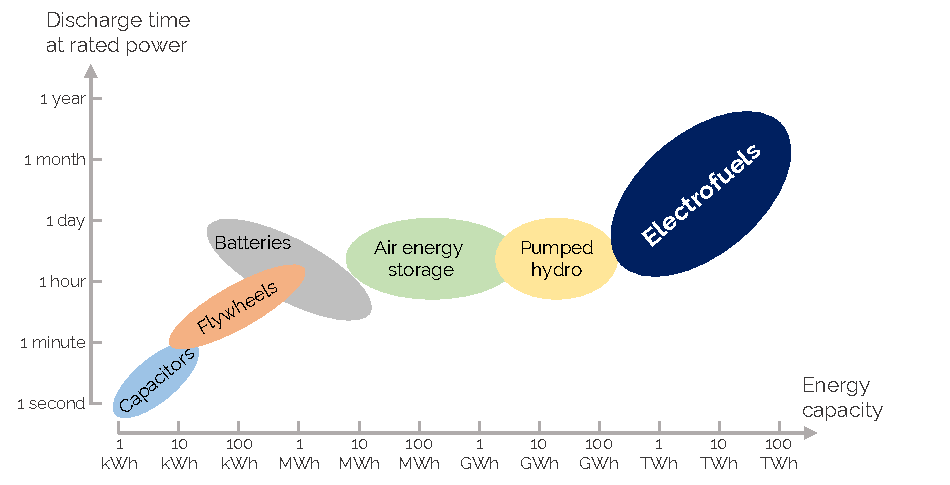
\includegraphics[width=0.9\textwidth]{Storage_electrofuels.pdf}
\caption{Energy carriers and technologies to store electricity. Electrofuels are an economical solution for high capacity and long-term storage of energy. Graph adapted from \cite{ISPT2017}.}
\label{fig:intro:Storage_electrofuels}
\end{figure}

To harvest the maximum potential of synthetic energy carriers in a sustainable transition and maximise the overall system efficiency \cite{mathiesen2015}, it is necessary to study the integration of these fuels within a multi-sector and whole-energy system \cite{Contino2020}. To reach this goal, an energy system optimisation model (ESOM) can define the design of the system to minimise, for instance, its costs or its emissions \cite{zeng2011review}. In this research field, \citet{yue2018review} highlighted that most of ESOMs use a deterministic approach (\ie 75\% out of the 134 reviewed ESOM studies). However, the model structures are inherently uncertain as well as their numerous composing parameters, especially when it comes to define an energy transition strategy for a large-scale system, such as a country. Given the lifetime of the conversion technologies, such strategy implies decisions with long-term impacts (20 to 50 years) where forecasts can be highly unreliable \cite{Moret2017}. Besides the uncertainty on the model structure (not addressed in this work), this long-term and large-system optimisation motivates the need to account for \gls{UQ} and consider it as a major challenge of such models \cite{pfenninger2014energy}. This challenge, along with a large number (\ie more than a hundred) of uncertain parameters and limited information of their distribution, leads to the "curse of dimensionality" \cite{kuo2005lifting}.


It aims at providing decision-makers with new methods and informed policies accounting for the intrinsic uncertainties of the future.  Instead of aiming at answering the question ``What could possibly happen in the future?'', let's rather address ``What could or should we do to make the future possible?'' ``Our task is not to foresee the future, but to enable it'' by Saint-Exupéry in Citadelle, 1948.



%!TEX root = ../thesis_main.tex
%!TEX encoding = UTF-8 Unicode

In their 2030 Agenda, United Nations have worked on identifying 17 \gls{SDGs} as a plan of action for society (or people), environment (or planet) and economy (or prosperity) \cite{un_sdgs}. 
%
%As Fatih
%
%On top of the depletion of (economically and environmentally) easy to harvest conventional fossil resources, the most urgent motivation for energy transition is the growing threat of climate change.  This change jeopardizes most of the \gls{SDGs} listed by the United Nations . Besides their environmental pillars (\ie 13-climate action, 14-life below water and 15-life on land)\cite{vinuesa2020role}, succeeding such a transition would contribute in reaching others of these goals like affordable 

From this need, develop a thread like I did in my FRIA application, we need whole-energy system model to give more insights to policymakers\\

Listing some examples of situations where uncertainties have not been considered and ended up in over-cost/waste of time/waste of..., highlight the need as well to consider uncertainties when we want to advise policymakers.\\

As the question of policymakers is not only what to do but how to do it, we need to address the optimisation of policies. This would introduce the RL part


\textbf{In a more sustainable future, some of the energy carriers, currently produced mostly from fossil resources, will still consist of hydrocarbons (\eg e-methane or e-methanol). This is why this paper rather uses ``defossilisation" rather than ``decarbonisation" as carbon will still play a key role in a carbon-neutral energy transition \cite{mertens2020carbon}.}



